\documentclass[aspectratio=169, 14pt]{beamer}
\usepackage[utf8]{inputenc}
\usepackage[english]{babel}
\usepackage{tipa}
\usepackage{graphicx}
\usepackage{transparent}
\usepackage[ruled, lined, linesnumbered, commentsnumbered]{algorithm2e}
\usepackage{pgfplots}
\newcommand\mycommfont[1]{\small\ttfamily\textcolor{blue}{#1}}
\SetCommentSty{mycommfont}
\renewcommand{\thealgocf}{}
\usepackage{setspace}
\usepackage{tikz}
\usetikzlibrary{matrix,backgrounds}
\usetikzlibrary{arrows}
\usetikzlibrary {arrows.meta}
\usetikzlibrary{calc,shadows.blur,fit,positioning}
\usetikzlibrary{shapes.multipart,chains}
\usepackage{minted}
\usepackage{fontawesome5}
\usepackage{booktabs}
\usepackage{caption}
\usepackage{bookmark}
\usepackage{hyperref}
\hypersetup{
    colorlinks=true,
    linkcolor=blue,
    filecolor=magenta,      
    urlcolor=cyan,
    }
\urlstyle{same}
\usetheme{metropolis}
\metroset{block=fill}
\usecolortheme{default}
\definecolor{darkmidnightblue}{rgb}{0.0, 0.2, 0.4}
\definecolor{LightGray}{gray}{0.9}


%------------------------------------------------------------
%This block of code defines the information to appear in the
%Title page
\title[Data Structures] %optional
{Data Structures}

\subtitle{Trees}

\author[CHEN Zhongpu] % (optional)
{CHEN Zhongpu}

\institute[] % (optional)
{
  School of Computing and Artificial Intelligence \\
  \href{mailto:zpchen@swufe.edu.cn}{zpchen@swufe.edu.cn}
}

\date[] % (optional)
{SWUFE, Fall 2022}

%End of title page configuration block
%------------------------------------------------------------


%------------------------------------------------------------
%The next block of commands puts the table of contents at the 
%beginning of each section and highlights the current section:

% \AtBeginSection[]
% {
%   \begin{frame}
%     \frametitle{Table of Contents}
%     \tableofcontents[currentsection]
%   \end{frame}
% }
%------------------------------------------------------------


\begin{document}

%The next statement creates the title page.
\frame{\titlepage}

%---------------------------------------------------------
%This block of code is for the table of contents after
%the title page
% \begin{frame}
% \frametitle{Table of Contents}
% \tableofcontents
% \end{frame}
%--------------------------------------------------------
\begin{frame}[fragile]
    \frametitle{Review}
    Linked lists and array-based lists work well for representing \alert{linear} relationships, but not all relationships are linear.


  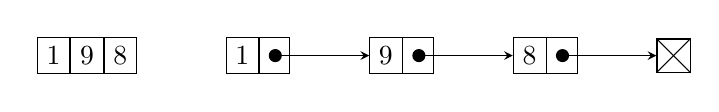
\begin{tikzpicture}[list/.style={rectangle split, rectangle split parts=2, draw, rectangle split horizontal}, >=stealth, start chain]
    \matrix[nodes=draw](array)
    {
      \node {1}; &
      \node {9}; &
      \node {8}; & \\
    };

  \node[list,on chain, right=of array] (A) {1};
  \node[list,on chain] (B) {9};
  \node[list,on chain] (C) {8};
  \node[on chain,draw,inner sep=6pt] (D) {};
  \draw (D.north east) -- (D.south west);
  \draw (D.north west) -- (D.south east);
  \draw[*->] let \p1 = (A.two), \p2 = (A.center) in (\x1,\y2) -- (B);
  \draw[*->] let \p1 = (B.two), \p2 = (B.center) in (\x1,\y2) -- (C);
  \draw[*->] let \p1 = (C.two), \p2 = (C.center) in (\x1,\y2) -- (D);

  \end{tikzpicture}

  \pause
\begin{block}{Example}
  Bob's father is Jack, and he has a sister named Alice. Which data structure can store those names and imply the relationships?
\end{block}
\end{frame}

\begin{frame}
In real word, we need to use \textbf{nonlinear} data structures. For example, items are often shown in a \alert{hierarchical} way, and such data structure is known as \alert{trees}.
    
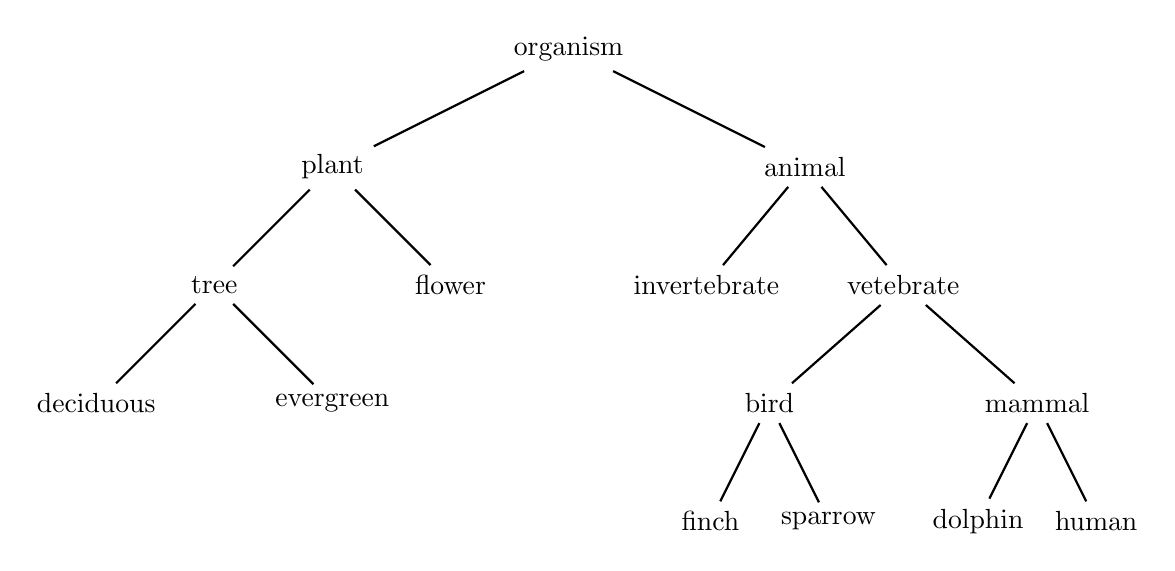
\begin{tikzpicture}
[sibling distance=6cm,-,thick,]
\node {organism}
  child {node {plant}
    [sibling distance=3cm]
    child {node {tree}
      child {node {deciduous}}
      child {node {evergreen}}
    }
    child {node {flower}}
  }
  child {node {animal}
    [sibling distance=2.5cm]
    child {node {invertebrate}}
    child {node {vetebrate}
      [sibling distance=3.4cm]
      child {node {bird}
        [sibling distance=1.5cm]
        child {node {finch}}
        child {node {sparrow}}
      }
      child {node {mammal}
        [sibling distance=1.5cm]
        child {node {dolphin}}
        child {node {human}}
      }
    }
  };
\end{tikzpicture}

\end{frame}

\begin{frame}

{\large \faIcon{code}} Try to write the HTML code based on its tag hierarchical structures.

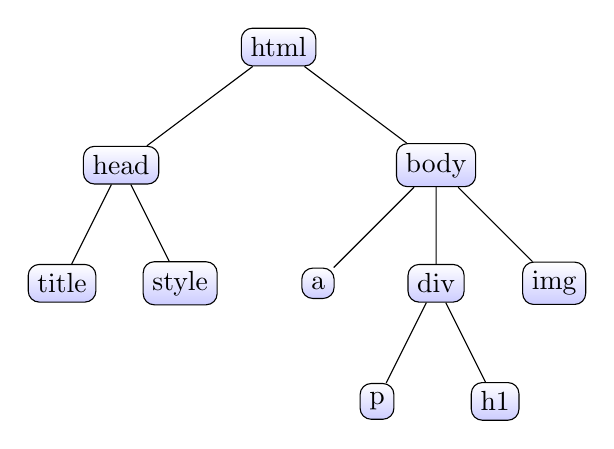
\begin{tikzpicture}[
  level 1/.style = {sibling distance = 4cm},
  level 2/.style = {sibling distance = 1.5cm},
every node/.style = {shape=rectangle, rounded corners,
  draw, align=center,
  top color=white, bottom color=blue!20}]
\node {html}
  child { node {head} 
      child {node {title} }
      child {node {style} }
  }
  child { node {body} 
      child {node {a} }
      child {node {div} 
          child {node {p}}
          child {node {h1}}
      }
      child {node {img} }
  };
\end{tikzpicture}
    

\end{frame}

{
    % \usebackgroundtemplate{\transparent{0.3}{\begin{picture}
    %     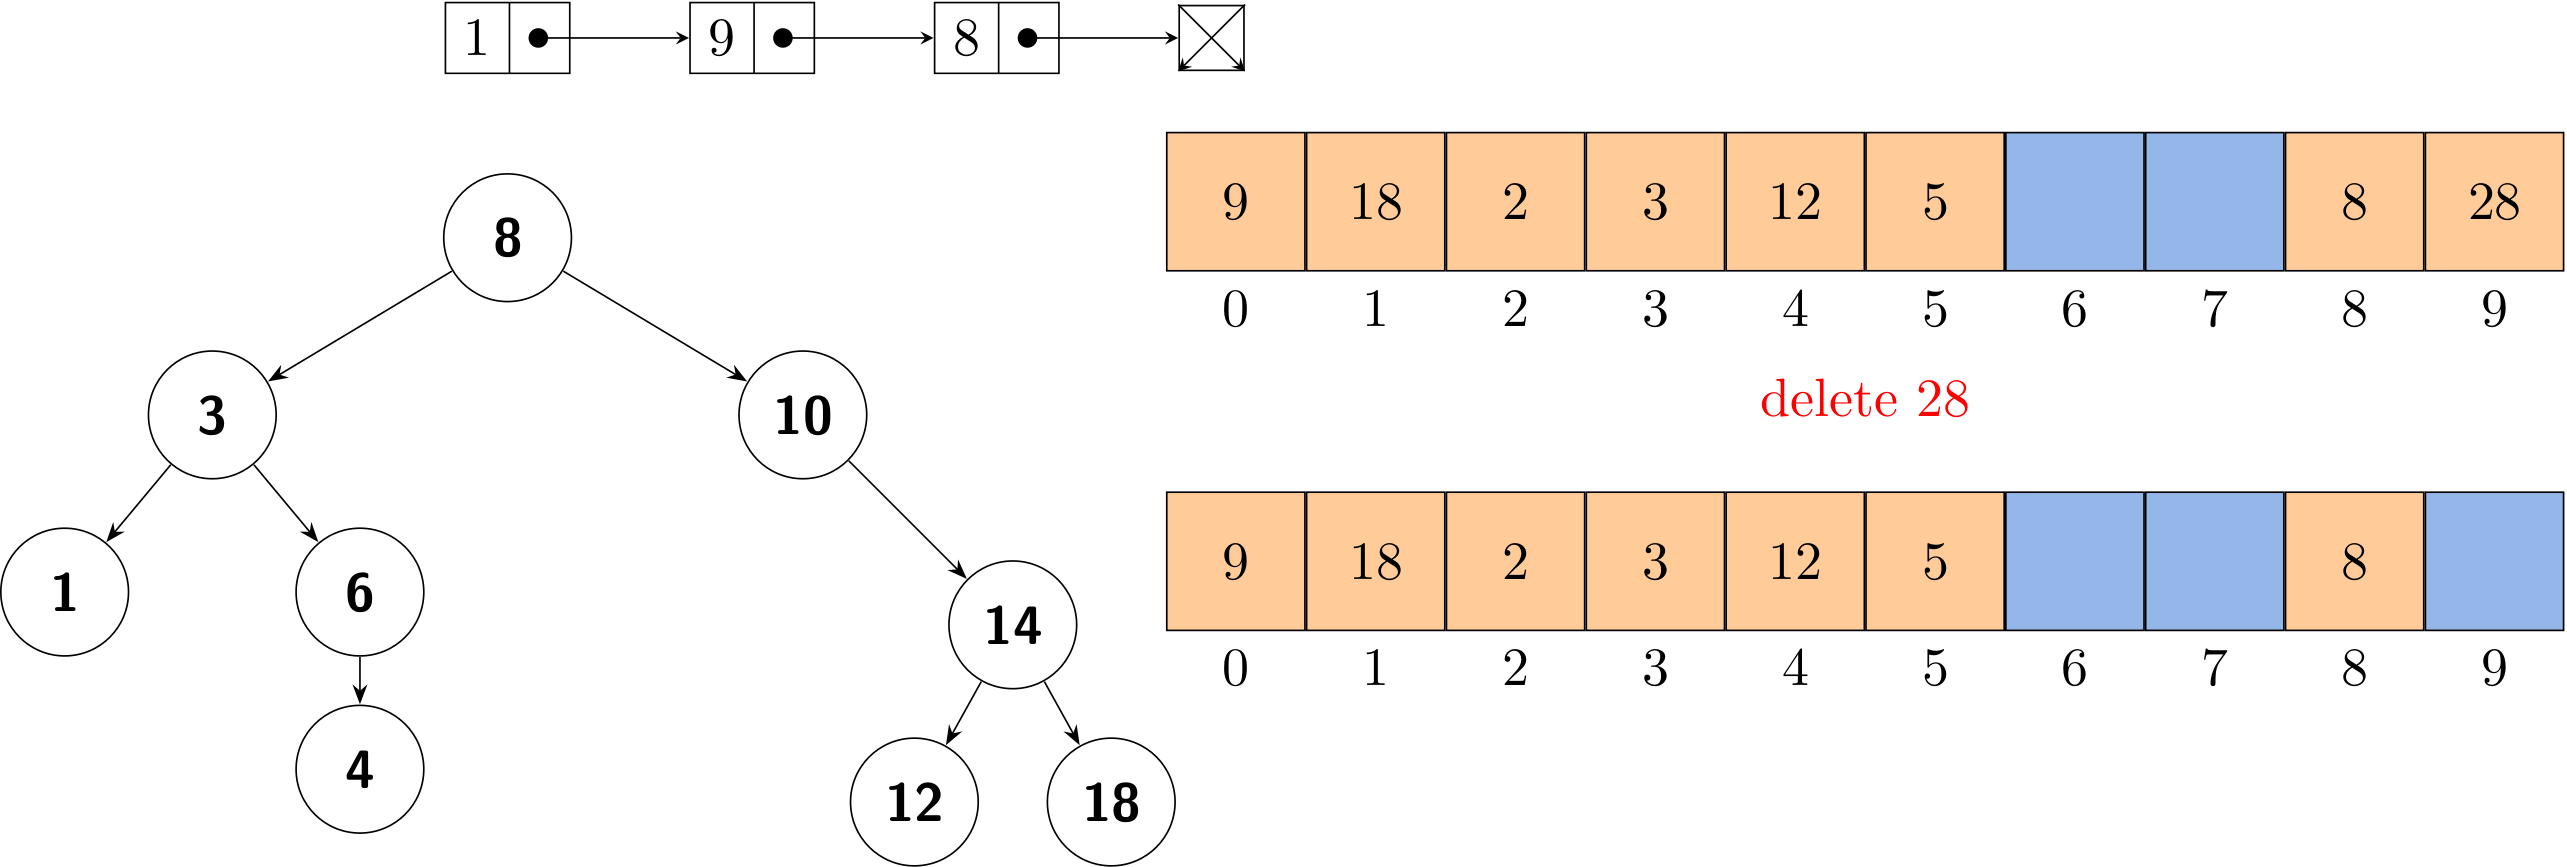
\includegraphics[height=0.7\paperheight]{cover}
    % \end{picture}    
    % }}
\usebackgroundtemplate{
  \tikz[overlay,remember picture] 
  \node[opacity=0.3, at=(current page.south east),anchor=south east, yshift=2cm,xshift=4cm] {
    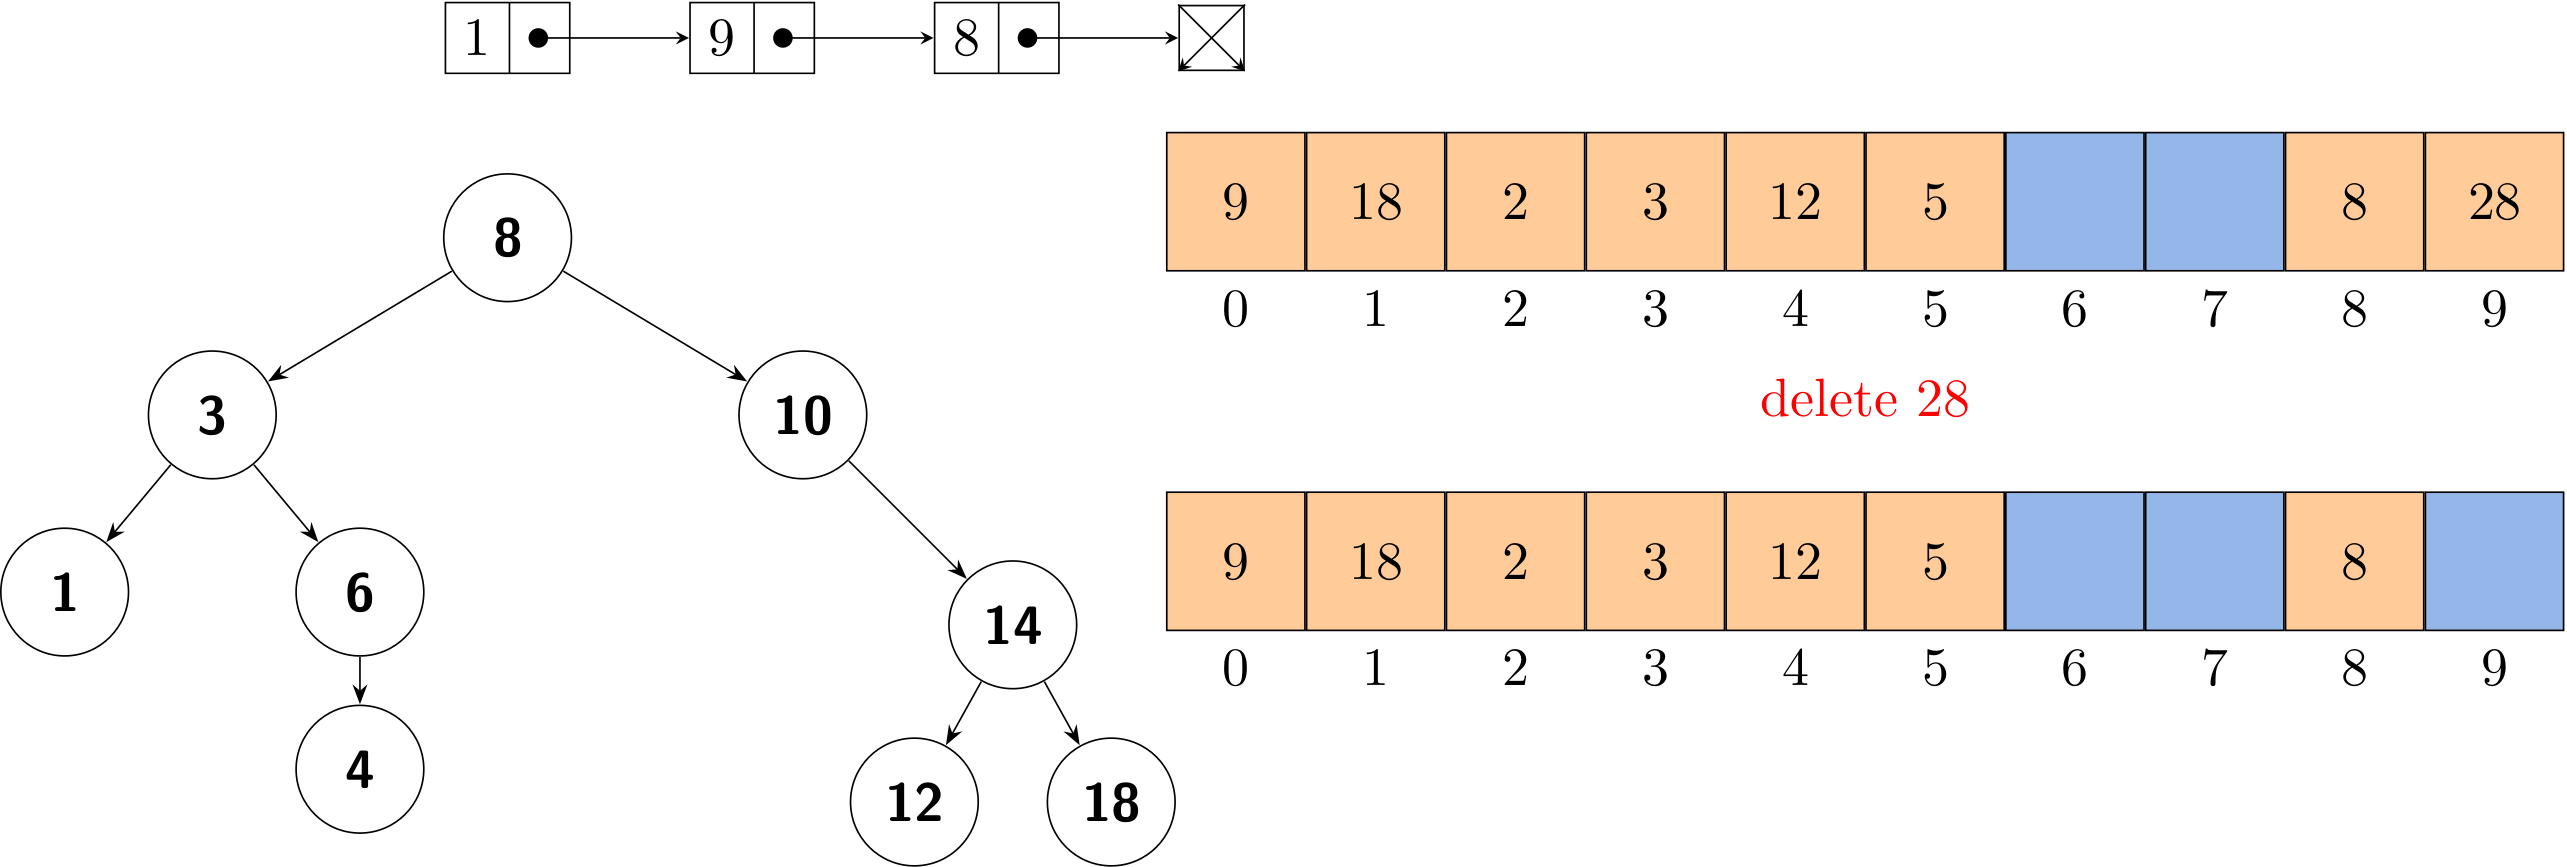
\includegraphics[height=0.6\paperheight]{cover}};
}
    \begin{frame}
        \section{\textcolor{darkmidnightblue}{1. Trees}}
    \end{frame}

}

\begin{frame}
  \frametitle{1.1 General Trees}
        \begin{exampleblock}{Tree}
          In computer science, a tree is a widely used ADT that represents a hierarchical tree structure with a set of connected nodes.
        \end{exampleblock}
  
  \begin{columns}
        \column{.35\textwidth}<1->
    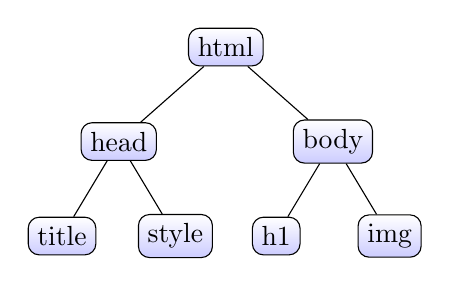
\begin{tikzpicture}[
  level 1/.style = {sibling distance = 3.4cm},
  level 2/.style = {sibling distance = 1.8cm},
every node/.style = {shape=rectangle, rounded corners,
  draw, align=center,
  top color=white, bottom color=blue!20}, scale=.8]
\node {html}
  child { node {head} 
      child {node {title} }
      child {node {style} }
  }
  child { node {body} 
      child {node {h1} }
      child {node {img} }
  };
\end{tikzpicture}
    \column{.65\textwidth}<2->
    This definition reveals that \textbf{parent-children} relationships are very important in trees.
  \end{columns}

\end{frame}

\begin{frame}

  A tree can be defined in a \textbf{recursive} way: a tree $T$ is either empty or consists of a node $r$, called the \alert{root} of $T$, and a (possibly empty) set of subtrees whose roots are the children of $r$.

  \begin{center}
        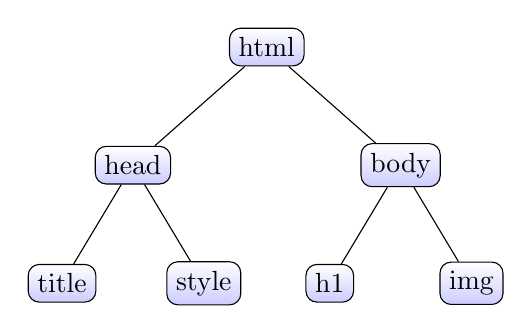
\begin{tikzpicture}[
  level 1/.style = {sibling distance = 3.4cm},
  level 2/.style = {sibling distance = 1.8cm},
every node/.style = {shape=rectangle, rounded corners,
  draw, align=center,
  top color=white, bottom color=blue!20}]
\node {html}
  child { node {head} 
      child {node {title} }
      child {node {style} }
  }
  child { node {body} 
      child {node {h1} }
      child {node {img} }
  };
\end{tikzpicture}
  \end{center}

\end{frame}

{\setbeamercolor{palette primary}{fg=black, bg=yellow}
\begin{frame}[standout]
  You have to known tons of terminologies while studying trees.

  \begin{itemize}
    \item \texttt{root}
    \item \texttt{link/edge}
    \item \texttt{parent}
    \item \texttt{child}
    \item \texttt{ancestor}
    \item ...
  \end{itemize}
\end{frame}
}

\begin{frame}[fragile]
  \frametitle{1.2 Terminologies}

  
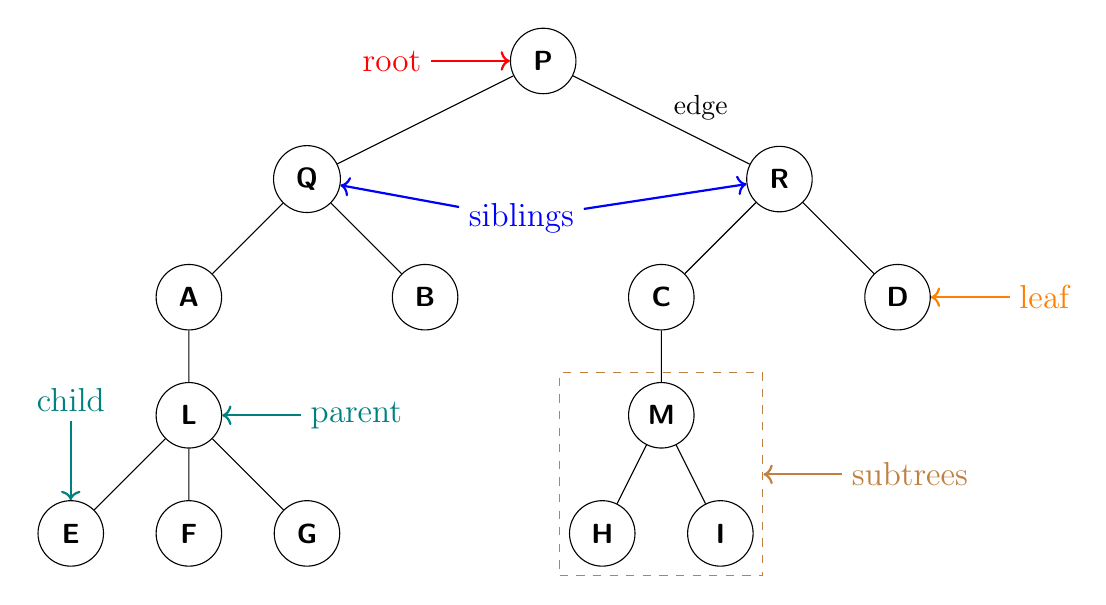
\begin{tikzpicture}[treenode/.style = {align=center, inner sep=1pt, text centered, font=\sffamily}, bst/.style = {treenode, circle, black, font=\sffamily\bfseries, draw=black, text width=2em},level/.style={sibling distance = 6cm/#1,
  level distance = 1.5cm}]
\node [bst] (rootn) {P}
    child {node [bst](nodeq) {Q}
        child {node [bst] {A}
          child {node [bst](nodel) {L}
            child {node [bst](nodee) {E}}
            child {node [bst] {F}}
            child {node [bst] {G}}
          }
        }
        child {node [bst] {B}}
    }
    child {node (noder) [bst, label={[xshift=-1.0cm, yshift=0.2cm]edge}] {R}
      child {node [bst] {C}
        child {node [bst] (nodem) {M}
          child {node [bst] (nodeh) {H}}
          child {node [bst] (nodei) {I}}
          }
      }
      child {node [bst](noded) {D}}
    }
;

\node[left=of rootn](roott) {\large \textcolor{red}{root}};
\draw[->, red, thick] (roott) -- (rootn);

\node[right=of nodeq, yshift=-.5cm, xshift=.5cm](siblingt) {\large \textcolor{blue}{siblings}};

\draw[->, blue, thick] (siblingt) -- (nodeq);
\draw[->, blue, thick] (siblingt) -- (noder);

\node[fit=(nodem)(nodei)(nodeh), dashed, draw, brown](subtrees) {};
\node[right=of subtrees](subtreest){\large \textcolor{brown}{subtrees}};
\draw[->, brown, thick] (subtreest) -- (subtrees);

\node[right=of nodel](parentt){\large \textcolor{teal}{parent}};
\draw[->, teal, thick] (parentt) -- (nodel);

\node[above=of nodee](childt){\large \textcolor{teal}{child}};
\draw[->, teal, thick] (childt) -- (nodee);

\node[right=of noded](leaft){\large \textcolor{orange}{leaf}};
\draw[->, orange, thick] (leaft) -- (noded);

\end{tikzpicture}

\end{frame}

\begin{frame}[fragile]

  \begin{columns}
    \column{.35\textwidth}
    A \textbf{path} is a sequence of nodes with the property that each node in the sequence is adjacent to the node linked to it. A path that does not repeat nodes is called a \textbf{simple path}.

    \column{.65\textwidth}
      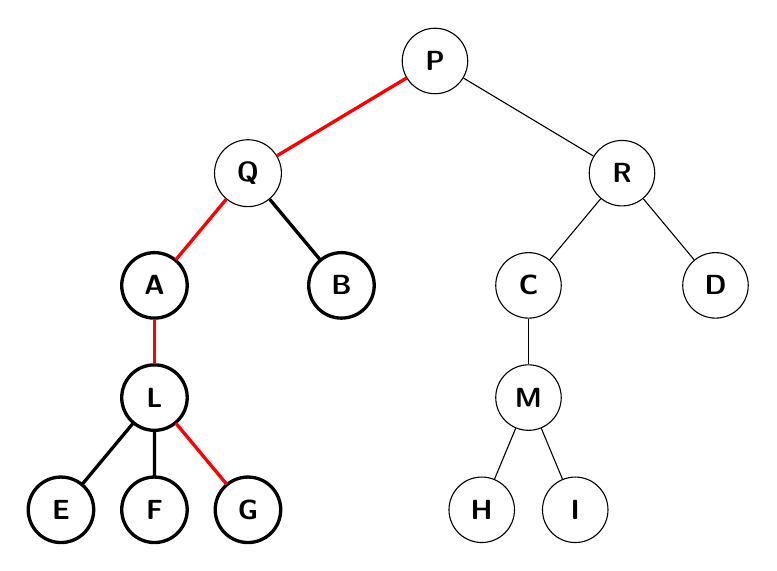
\begin{tikzpicture}[treenode/.style = {align=center, inner sep=1pt, text centered, font=\sffamily}, bst/.style = {treenode, circle, black, font=\sffamily\bfseries, draw=black, text width=2em},level/.style={sibling distance = 5cm/#1,
    level distance = 1.5cm}, scale=.95, redline/.style = {edge from parent/.style={draw, red, very thick}}, blackline/.style={edge from parent/.style={draw, black}}]
  \node [bst] (rootn) {P}
      child[redline] {node [bst](nodeq) {Q}
          child {node [bst] {A}
            child {node [bst](nodel) {L}
              child[blackline] {node [bst](nodee) {E}}
              child[blackline] {node [bst] {F}}
              child {node [bst] {G}}
            }
          }
          child[blackline] {node [bst] {B}}
      }
      child {node (noder) [bst] {R}
        child {node [bst] {C}
          child {node [bst] (nodem) {M}
            child {node [bst] (nodeh) {H}}
            child {node [bst] (nodei) {I}}
            }
        }
        child {node [bst](noded) {D}}
      }
  ;
  \end{tikzpicture}
  \end{columns}

\end{frame}

\begin{frame}[fragile]

  \begin{columns}
    \column{.35\textwidth}
      The \textbf{height} of a node is the length of the longest downward path to a leaf from that node. 
      \[height(root) = height(T)\]
      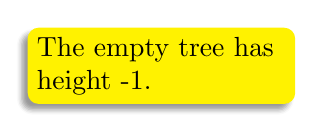
\begin{tikzpicture}
    \node[fill=yellow,blur shadow={shadow xshift=-0.5ex},
    text width=9em,anchor=south west,rounded corners]
    {The empty tree has height -1.};
    \end{tikzpicture}
    \column{.65\textwidth}
      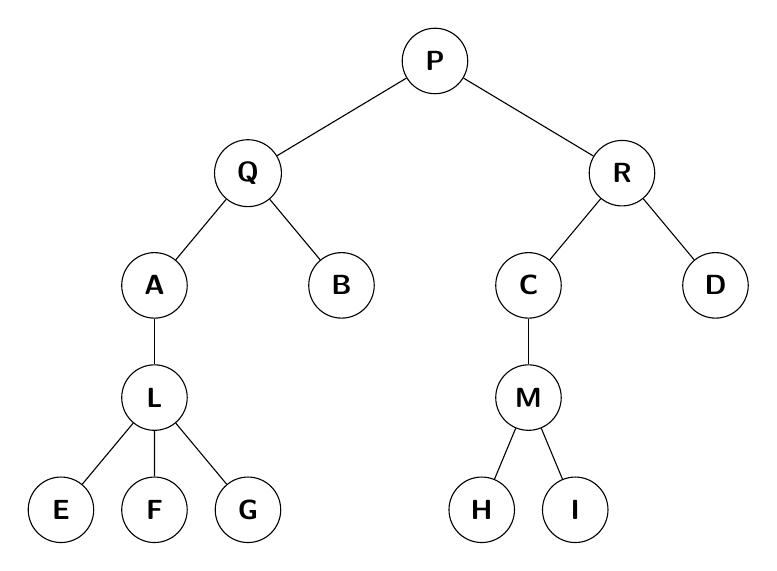
\begin{tikzpicture}[treenode/.style = {align=center, inner sep=1pt, text centered, font=\sffamily}, bst/.style = {treenode, circle, black, font=\sffamily\bfseries, draw=black, text width=2em},level/.style={sibling distance = 5cm/#1,
    level distance = 1.5cm}, scale=.95]
  \node [bst] (rootn) {P}
      child {node [bst](nodeq) {Q}
          child {node [bst] {A}
            child {node [bst](nodel) {L}
              child {node [bst](nodee) {E}}
              child {node [bst] {F}}
              child {node [bst] {G}}
            }
          }
          child {node [bst] {B}}
      }
      child {node (noder) [bst] {R}
        child {node [bst] {C}
          child {node [bst] (nodem) {M}
            child {node [bst] (nodeh) {H}}
            child {node [bst] (nodei) {I}}
            }
        }
        child {node [bst](noded) {D}}
      }
  ;
  \end{tikzpicture}
  \end{columns}
        
\end{frame}

\begin{frame}[fragile]
  \frametitle{1.3 Revisit Nodes}

  Generally, every node has links to its parent and children, and holds a \alert{key} and an associated \alert{value} (aka \textbf{satellite data}).

  \begin{minted}[bgcolor=LightGray, baselinestretch=1]{python}
class Node:
  def __init__(self, parent, children, key, value):
      self._parent = parent
      self._children = children
      self._key = key
      self._value = value
  \end{minted}

But, for simplicity, we only consider \textbf{keys}.
\end{frame}

\begin{frame}

        \section{\textcolor{darkmidnightblue}{2. Binary Search Trees}} 

\end{frame}

\begin{frame}[fragile]
  \frametitle{2.1 Binary Trees}

  \begin{columns}
    \column{.6\textwidth}

  \begin{block}{Binary Trees}
    Each node has \emph{exactly two links}, which are called its \textbf{left} and \textbf{right} links, that point to nodes called its \alert{left child} and \alert{right child}, respectively.
  \end{block}
    \column{.4\textwidth}
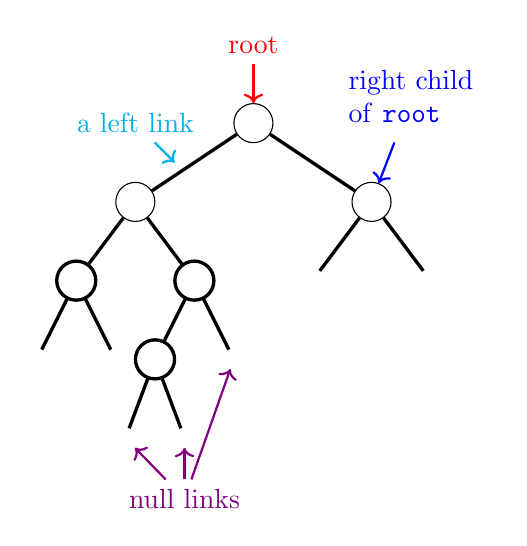
\begin{tikzpicture}[treenode/.style = {align=center, inner sep=1pt, text centered, font=\sffamily}, bst/.style = {treenode, circle, black, font=\sffamily\bfseries, draw=black, text width=1.2em}, level/.style={sibling distance = 3cm/#1, level distance = 1cm}, edge from parent/.style={draw, very thick}]

  \node[bst] (root) {}
    child {node[bst](leftn) {}
      child {node[bst] {}
        child {node {}}
        child {node {}}
      }
      child {node[bst] {}
        child {node[bst] {}
          child {node(null1) {}}
          child {node(null2) {}}
          }
        child {node(null3) {}}
      }
    }
    child {node[bst] (rightn) {}
      child {node {}}
      child {node {}}
    }
  ;
  \node[above=of root, yshift=-.5cm](roott) {\textcolor{red}{root}};
  \draw[->, thick, red] (roott) -- (root);

  \node[above=of rightn, xshift=.5cm,yshift=-.5cm, align=left](rightt) {\begin{tabular}{l}
    \textcolor{blue}{right child} \\
    \textcolor{blue}{of \texttt{root}}
\end{tabular}};
\draw[->, blue, thick] (rightt) -- (rightn);

\node[above=of leftn, yshift=-.5cm](leftt){\textcolor{cyan}{a left link}};

\draw[->, thick, cyan] (leftt) -- (-1, -.5);

\node[below=of null2, yshift=.6cm](nullt){\textcolor{violet}{null links}};
\draw[->, thick, violet] (nullt) -- (null1);

\draw[->, thick, violet] (nullt) -- (null2);
\draw[->, thick, violet] (nullt) -- (null3);


\end{tikzpicture}
  \end{columns}

\end{frame}

\begin{frame}
  \frametitle{2.2 Binary Search Trees}

  \begin{block}{Binary Search Trees}
    A binary search tree (BST) is a binary tree where each node has a (comparable) key and satisfies the restriction that the key in any node is larger than the keys in all nodes in that node's left subtree and smaller than the keys in all nodes in that node's right subtree.
  \end{block}

  \pause
  The \alert{binary-search-tree property}: Let $x$ be a node in a BST.

  \begin{itemize}
    \item If $y$ is a node in the left subtree of $x$, then $y.key < x.key$.
    \item If $y$ is a node in the right subtree of $x$, then $y.key > x.key$.
  \end{itemize}
\end{frame}

\begin{frame}[fragile]

  \begin{center}
      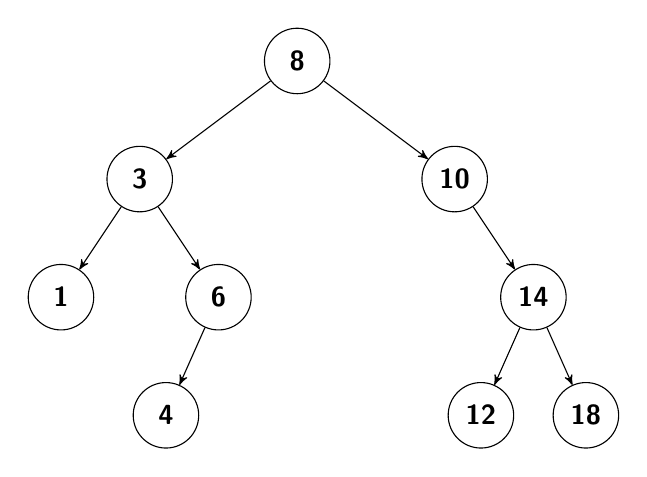
\begin{tikzpicture}[treenode/.style = {align=center, inner sep=1pt, text centered,
    font=\sffamily},
  bst/.style = {treenode, circle, black, font=\sffamily\bfseries, draw=black, text width=2em}, ->,>=stealth',level/.style={sibling distance = 4cm/#1,
  level distance = 1.5cm}]
\node [bst] {8}
    child {node [bst] {3}
        child {node [bst] {1}}
        child {node [bst](n6) {6}
            child {node [bst] {4}}
            child[edge from parent/.style={draw=none}] {node {}}
        }
    }
    child {node (n10) [bst] {10}
       child[edge from parent/.style={draw=none}] {node {}}
        child {node [bst] {14}
            child {node [bst] {12}}
            child {node [bst] {18}}
        }
    }
;
\end{tikzpicture}
  \end{center}


    Thanks to the \alert{binary-search-tree property}, it supports efficient search. For instance, how to search 6?

\end{frame}

\begin{frame}[fragile]
  \frametitle{Exercise}

  {\large \faIcon{question-circle}} Is it a BST?

        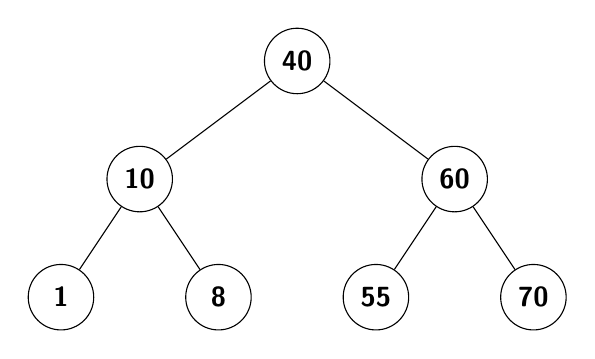
\begin{tikzpicture}[treenode/.style = {align=center, inner sep=1pt, text centered,
    font=\sffamily},
  bst/.style = {treenode, circle, black, font=\sffamily\bfseries, draw=black, text width=2em},level/.style={sibling distance = 4cm/#1,
  level distance = 1.5cm}]
\node [bst] {40}
    child {node [bst] {10}
        child {node [bst] {1}}
        child {node [bst](n6) {8}}
    }
    child {node [bst] {60}
       child {node[bst] {55}}
        child {node [bst] {70}
        }
    }
;
\end{tikzpicture}
\end{frame}

\begin{frame}[fragile]
  \frametitle{2.3 BST: structure}

  \begin{columns}
        \column{.55\textwidth}
      \begin{minted}[bgcolor=LightGray, fontsize=\small]{python}
class Node:
    def __init__(self, key, 
            left=None, right=None):
        self.key = key
        self.left = left
        self.right = right

class BST:
    def __init__(self):
        self.root = None     
    \end{minted}
    \column{.45\textwidth}
    A node in a BST consists of
\begin{itemize}
  \item a link to its left subtree
  \item a link to its right subtree
  \item the key
  \item the value
\end{itemize}

  \end{columns}

\end{frame}

\begin{frame}[fragile]
  \frametitle{2.4 BST: get()}
This method is often called \texttt{search()}. It is used to get the node containing the given key.

\begin{columns}
  \column{.5\textwidth}<1->
  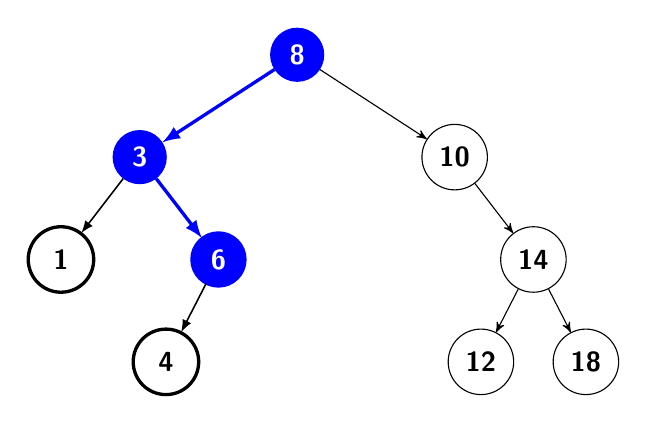
\begin{tikzpicture}[treenode/.style = {align=center, inner sep=1pt, text centered,
    font=\sffamily},
  bst/.style = {treenode, circle, black, font=\sffamily\bfseries, draw=black, text width=2em}, ->,>=stealth',level/.style={sibling distance = 4cm/#1,
  level distance = 1.3cm}, bluebst/.style = {treenode, circle, white, font=\sffamily\bfseries, draw=blue, fill=blue, text width=1.5em},
orangebst/.style = {treenode, circle, white, font=\sffamily\bfseries, draw=orange, fill=orange, text width=1.5em},
blueline/.style={edge from parent/.style={blue,very thick,-latex,draw}},
orangeline/.style={edge from parent/.style={orange,very thick,-latex,draw}},
commonline/.style={edge from parent/.style={black,line width=0.2mm,-latex,draw}}]
\node [bluebst] {8}
    child[blueline] {node [bluebst] {3}
        child[commonline] {node [bst] {1}}
        child {node [bluebst] {6}
            child[commonline] {node [bst] {4}}
            child[edge from parent/.style={draw=none}] {node {}}
        }
    }
    child {node (n10) [bst] {10}
       child[edge from parent/.style={draw=none}] {node {}}
        child {node [bst] {14}
            child {node [bst] {12}}
            child {node [bst] {18}}
        }
    }
;
\end{tikzpicture}
    
  \column{.5\textwidth}<2->
  {\large \faIcon{lightbulb}} The core idea: starting from \texttt{root}, trace a simple path downward in the tree until meeting the \texttt{key} or \texttt{null}.
\end{columns}

\end{frame}

\begin{frame}

  \scalebox{.8}{  
    \begin{algorithm}[H]
    \caption{get(key)}
    $x\gets root$ \\
\While{x $\neq$ null and x.key $\neq$ key}{
    \If{key $<$ x.key}{
        $x\gets x.left$
    }\Else{
        $x\gets x.right$
    }
}
\Return{x}
\end{algorithm}
}

\pause
{\large \faIcon{question-circle}} What is the time complexity of \texttt{get()}?

{\large \faIcon{question-circle}} How to implement \texttt{contains()} based on \texttt{get()}?
\end{frame}

\begin{frame}[fragile]
  \frametitle{2.5 BST: put()}
This method is often called \texttt{insert()}. It is used to insert a new key.
  
\begin{columns}
  \column{.5\textwidth}<1->
  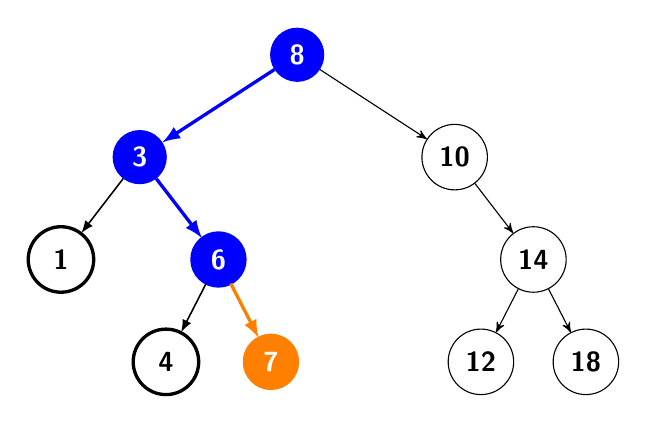
\begin{tikzpicture}[treenode/.style = {align=center, inner sep=1pt, text centered,
    font=\sffamily},
  bst/.style = {treenode, circle, black, font=\sffamily\bfseries, draw=black, text width=2em}, ->,>=stealth',level/.style={sibling distance = 4cm/#1,
  level distance = 1.3cm}, bluebst/.style = {treenode, circle, white, font=\sffamily\bfseries, draw=blue, fill=blue, text width=1.5em},
orangebst/.style = {treenode, circle, white, font=\sffamily\bfseries, draw=orange, fill=orange, text width=1.5em},
blueline/.style={edge from parent/.style={blue,very thick,-latex,draw}},
orangeline/.style={edge from parent/.style={orange,very thick,-latex,draw}},
commonline/.style={edge from parent/.style={black,line width=0.2mm,-latex,draw}}]
\node [bluebst] {8}
    child[blueline] {node [bluebst] {3}
        child[commonline] {node [bst] {1}}
        child {node [bluebst] {6}
            child[commonline] {node [bst] {4}}
            child[orangeline] {node[orangebst] {7}}
        }
    }
    child {node (n10) [bst] {10}
       child[edge from parent/.style={draw=none}] {node {}}
        child {node [bst] {14}
            child {node [bst] {12}}
            child {node [bst] {18}}
        }
    }
;
\end{tikzpicture}
    
  \column{.5\textwidth}<2->
  {\large \faIcon{lightbulb}} The core idea: it works like \texttt{get()} by inserting the new key as a leaf node.
\end{columns}
\end{frame}

\begin{frame}

  \scalebox{.8}{  
    \begin{algorithm}[H]
      \setstretch{.9}
    \caption{put(key)}
    $z\gets Node(key)$ \\
    $x\gets root$ \\
    $y\gets null$ \\
    \While{x $\neq$ null}{
        $y\gets x$ \\
        \uIf{key $<$ x.key}{
            $x\gets x.left$
        }\uElseIf{key $>$ x.key}{
            $x\gets x.right$ 
        }\uElse{
            \Return{}
        }
    }
    \uIf{y == null}{
        $root\gets z$
    }\uElseIf{key $<$ y.key}{
        $y.left\gets z$
    }\uElse{
        $y.right\gets z$
    }
    \end{algorithm}
}

\end{frame}

\begin{frame}
  \frametitle{Exercise}
{\large \faIcon{pen-fancy}} Please draw the BST after inserting 5, 2, 4, 10, 8, 7, 42, in that order into an empty BST.

\end{frame}

\begin{frame}
  \frametitle{2.6 Recursive get()}
\begin{itemize}
  \item \textbf{Base step}: \texttt{key} is found or reaching \texttt{null}.
  \item \textbf{Recursive step}: get from its left or right subtree.
\end{itemize}  

\scalebox{.8}{  
  \begin{algorithm}[H]
    \setstretch{1.1}
    \caption{get(x, key)}
    \If{x == null or key == x.key}{
        \Return{x}
    }
    \If{key $<$ x.key}{
        \Return{get(x.left, key)}
    }\Else{
        \Return{get(x.right, key)}
    }
    \end{algorithm}
}

\end{frame}

\begin{frame}
  \frametitle{2.7 Recursive put()}
\texttt{put(x, key)}: to insert a new \texttt{key} into a BST rooted at \texttt{x}, and then return the root. 

\scalebox{.8}{  
  \begin{algorithm}[H]
    \setstretch{1}
    \caption{put(x, key)}
    \If{x == null}{
        \Return{Node(key)}
    }
    \If{key $<$ x.key}{
        $x.left\gets put(x.left, key)$
    } \ElseIf{key $>$ x.key} {
        $x.right\gets put(x.right, key)$
    }
    \Return{x}
    \end{algorithm}
}

\end{frame}

{\setbeamercolor{palette primary}{fg=black, bg=yellow}
\begin{frame}[standout]
  Generally, recursive implementations are a bit easier to verify for correctness; non-recursive implementations are a bit more efficient.
\end{frame}
}

\begin{frame}
  \frametitle{Exercise}
{\large \faIcon{code}} How to count the number of nodes (i.e., \texttt{size()}) in a BST using a recursive implementation?

\end{frame}

\begin{frame}[fragile]
  \frametitle{2.8 Ordered-based Operations}

A BST supports a myriad of ordered-based operations, such as \texttt{min()}, \texttt{max()}, \texttt{floor()}, and \texttt{ceiling()};

  
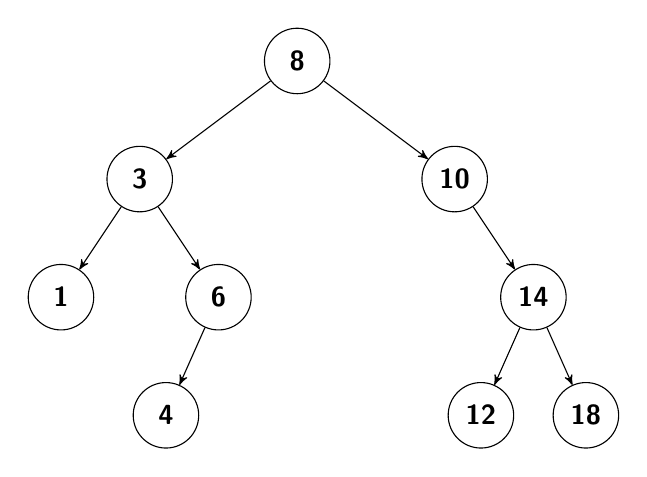
\begin{tikzpicture}[treenode/.style = {align=center, inner sep=1pt, text centered,
  font=\sffamily},
bst/.style = {treenode, circle, black, font=\sffamily\bfseries, draw=black, text width=2em}, ->,>=stealth',level/.style={sibling distance = 4cm/#1,
level distance = 1.5cm}]
\node [bst] {8}
  child {node [bst] {3}
      child {node [bst] {1}}
      child {node [bst](n6) {6}
          child {node [bst] {4}}
          child[edge from parent/.style={draw=none}] {node {}}
      }
  }
  child {node (n10) [bst] {10}
     child[edge from parent/.style={draw=none}] {node {}}
      child {node [bst] {14}
          child {node [bst] {12}}
          child {node [bst] {18}}
      }
  }
;
\end{tikzpicture}

\end{frame}

\begin{frame}
  \frametitle{max()}
Note that the maximum key is always located at the \textbf{rightmost} in a BST.

\scalebox{.8}{  
  \begin{algorithm}[H]
    \setstretch{1}
    \caption{max()}
    \If{root == null} {
      throw NoSuchElement Error
    }
    $x\gets root$ \\
    \While{x.right $\neq$ null} {
      $x\gets x.right$
    }
    \Return{x.key}
    \end{algorithm}
}

\end{frame}

\begin{frame}[fragile]
The recursive implementation of \texttt{max()}:

\scalebox{.8}{  
  \begin{algorithm}[H]
    \setstretch{1}
    \caption{max(x)}
    \If{x.right == null} {
      \Return{x}
    } \Else {
      \Return{max(x.right)}
    }
    \end{algorithm}
}

\begin{minted}[bgcolor=LightGray]{java}
if (root == null) {
  throw new NoSuchElementException();
}
return max(root).key;
      \end{minted}
\end{frame}

\begin{frame}
  \frametitle{Exercise}
  
  {\large \faIcon{code}} Please implement \texttt{min()} in a recursive and an iterative way, respectively.
\end{frame}

\begin{frame}[fragile]
  \frametitle{removeMin()}
To remove the node with the minimum key. Note that it is always located at the \textbf{leftmost} in a BST.

\begin{columns}
  \column{.45\textwidth}<1->
  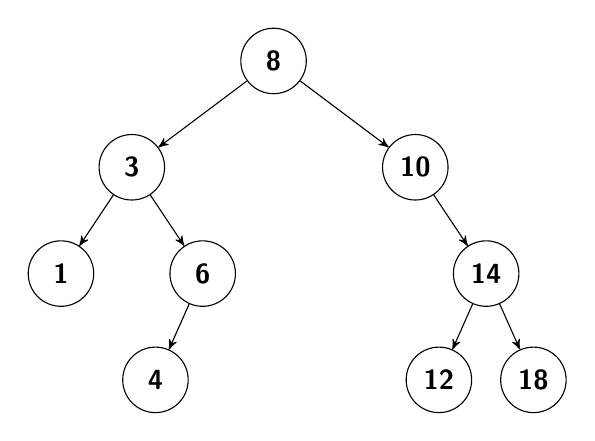
\begin{tikzpicture}[treenode/.style = {align=center, inner sep=1pt, text centered,
    font=\sffamily},
  bst/.style = {treenode, circle, black, font=\sffamily\bfseries, draw=black, text width=2em}, ->,>=stealth',level/.style={sibling distance = 4cm/#1,
  level distance = 1.5cm}, scale=.9]
  \node [bst] {8}
    child {node [bst] {3}
        child {node [bst] {1}}
        child {node [bst](n6) {6}
            child {node [bst] {4}}
            child[edge from parent/.style={draw=none}] {node {}}
        }
    }
    child {node (n10) [bst] {10}
       child[edge from parent/.style={draw=none}] {node {}}
        child {node [bst] {14}
            child {node [bst] {12}}
            child {node [bst] {18}}
        }
    }
  ;
  \end{tikzpicture}
  \column{.55\textwidth}<2->
  \alert{\texttt{removeMin(x)}}: it takes a node \texttt{x} then returns a root of the subtree rooted at \texttt{x} after removing the node with the smallest key.
\end{columns}

\end{frame}

\begin{frame}
\begin{itemize}
  \item \textbf{Base step}: if $x.left$ is \texttt{null}, return its right child.
  \item \textbf{Recursive step}: otherwise, update $x.left$ to \texttt{removeMin(x.left)}.
\end{itemize}

\scalebox{.8}{  
  \begin{algorithm}[H]
    \caption{removeMin(x)}
    \If{x.left = null}{
      \Return{x.right}
  }
  $x.left\gets removeMin(x.left)$ \\
  \Return{x}    
    \end{algorithm}
}
\end{frame}

\begin{frame}

  \scalebox{.8}{  
    \begin{algorithm}[H]
      \setstretch{1.1}
      \caption{removeMin()}
      \If{root == null}{throw NoSuchElement error}
      $x\gets root$ \\
      $y\gets null$ \\ 
      \While{x.left $\neq$ null}{
      $y\gets x$ \\
      $x\gets x.left$ 
      }
      \If{y == null}{
          $root\gets x.right$
      }\Else{
          $y.left\gets x.right$
      } 
      \end{algorithm}
  }

\end{frame}

\begin{frame}
  
  \section{\textcolor{darkmidnightblue}{Conclusion}} 

  \begin{enumerate}
    \item Trees
    \item Binary search trees
    \item BST: search and insert
    \item Recursive and iterative algorithms on a BST
  \end{enumerate}
\end{frame}

\begin{frame}
  \frametitle{This Week's Task}
\begin{itemize}
  \item Implement a BST using Python or Java.
  \item Try to implement \texttt{floor()} and \texttt{ceiling()} for BSTs.
\end{itemize}  

\end{frame}

\end{document}